\documentclass[12pt]{article}
\usepackage{graphicx,multicol,lipsum}
\title{Generative Advereial Network}
\author{Harshal Patel\\2019pcp5048 MNIT Jaipur}
\date{October, 2019}

\begin{document}
\maketitle
\section*{Abstract}
Earlier neural networks are only used for classification , regression and object detection only but using generative neural network computer can generate artificial images, Aim of this paper is to provide an basic information about what genrative adverserial network is and where they are used.

\begin{multicols}{2}
\section{Introduction}
In generative neural network instead of training only one neural network, we are training two neural networks one for generating artifical images and one for detecting whether image came from original input set or from generator.It is like minimax game. Purpose of Generator is to maximize probability of Descriminator making mistake.
It can be seen as counterfeiters, trying to make fake currency and cop trying to detect it.
Generator and descriminator are trained using multilayer perceptron by backpropogation .

\section{Applications}
GANs are trained on wide range of datasets from MNIST[], toronto face detection [], and CIFAR[].
Generator network uses linear and sigmoid activation functions while descriminator uses maxout activation. dropout technique is used to remove neurons in order to avoid overfitting. 


\end{multicols}
\begin{table}
\begin{tabular}{ c | c | c } 
 \hline
\textbf{Model} & \textbf{MNIST} & \textbf{TFD}\\
 \hline\hline
 DBN & 138±2 & 1909±66\\

Deep GSN & 121±1.6 & 2110±50\\
Adverserial Nets & 225±2 & 2017±26


\end{tabular}
\caption{Parzen window-based log-likelihood estimates. The reported numbers on MNIST are the mean loglikelihood of samples on test set, with the standard error of the mean computed across examples}
\end{table}

%This is just to test
\begin{multicols}{2}
\lipsum[1]
\end{multicols}
%just to test ends here


\begin{figure}
\centering
\begin{minipage}{.45\textwidth}
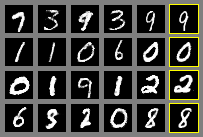
\includegraphics[width=\textwidth]{mnist1.png}
\caption{mnist dataset}
\end{minipage}
~~~~
\begin{minipage}{.45\textwidth}
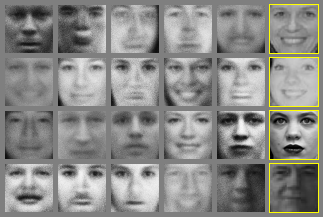
\includegraphics[width=\textwidth]{tfd1.png}
\caption{TFD dataset}
\end{minipage}
\end{figure}


\end{document}